\documentclass[10pt,a5paper]{article}
\renewcommand{\baselinestretch}{1.0}
\usepackage{cite}
\usepackage[dvips]{graphicx}
\usepackage{psfrag}
\usepackage{color}
\usepackage[cmex10]{amsmath}
\usepackage{amsfonts}
\usepackage[font=footnotesize, captionskip=10pt]{subfig}
\usepackage{tikz}
\usepackage{flushend}
\usepackage{times}
\usepackage[margin=1.5cm]{geometry}

\usepackage[slovak]{babel}
\usepackage[utf8]{inputenc}
\usepackage[T1]{fontenc}

\pagestyle{empty}

\hyphenation{net-works}
\newtheorem{remark}{Remark}

\begin{document}

\title{Paper title}
\author{Michal Chovanec\\
michal.chovanec@yandex.com}
\date{}
\maketitle
\thispagestyle{empty}

%\noindent$^1$\ affiliation\\
%\noindent$^2$\ affiliation\\

\noindent {\bf Keywords:} keywords...

\noindent {\bf Abstract:} Abstract

\section{Introduction}

Úvod ~\cite{bib:Aproximation}.
ľ š ť ž  \\
č ý á í é ú ä ô ň \\

\begin{equation}
\label{McCulloch_Pitts}
  y(n) = \varphi(\sum_{i = 0}^{N-1} x_i(n)w_i(n))
\end{equation}


\section{Experimental results}

yeah, fucking awesome, many pictures == many pages to be taken

\begin{figure}[!ht]
\centering
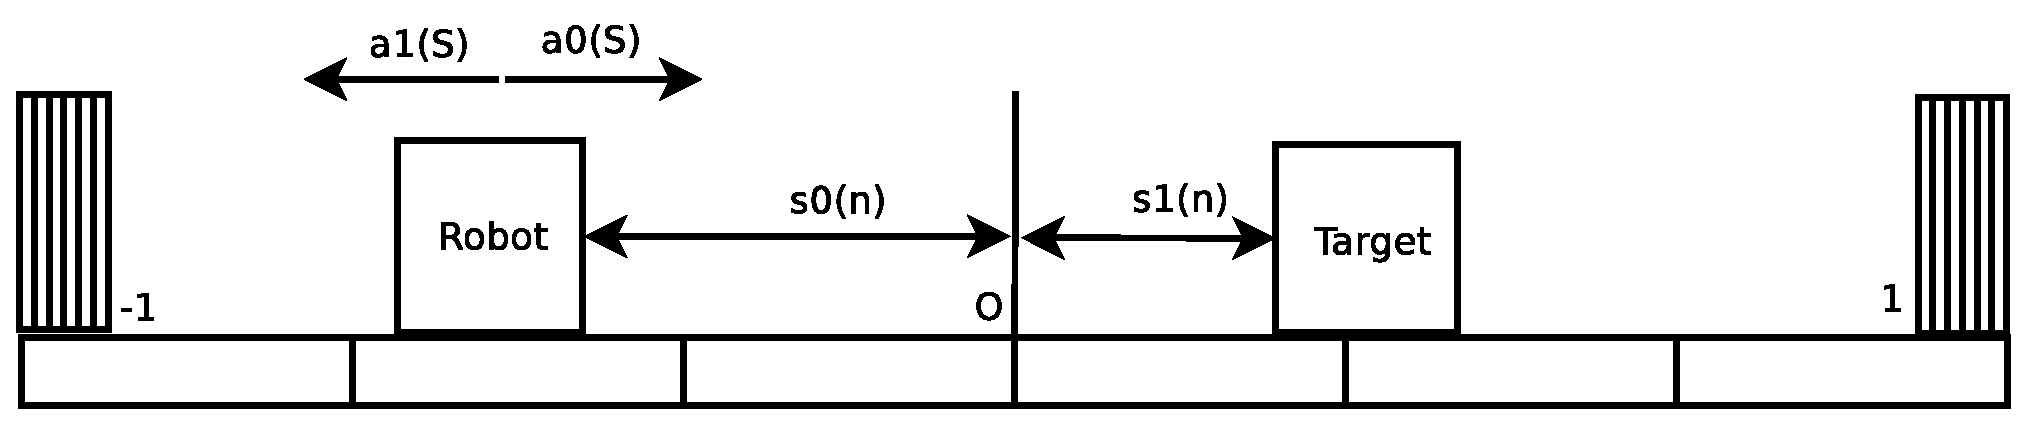
\includegraphics[width=3.0in]{q_learning_test/pictures/1D_robot_diagram.eps}
\caption{experiment schematic}
\label{experiment schematic}
\end{figure}

\subsection{Experiment 1}

all for k = 1.1

\begin{figure}[!ht]
\centering
\includegraphics[width=2.9in]{q_learning_test/experiment_01/table/q_map.png}
\caption{table Q max value}
\label{table Q max value}
\end{figure}

\begin{figure}[!ht]
\centering
\includegraphics[width=2.9in]{q_learning_test/experiment_01/table/q_action_id.png}
\caption{table action id}
\label{table action id}
\end{figure}

\begin{figure}[!ht]
\centering
\includegraphics[width=2.9in]{q_learning_test/experiment_01/table/q_action.png}
\caption{table action value}
\label{table action value}
\end{figure}

\begin{figure}[!ht]
\centering
\includegraphics[width=2.9in]{q_learning_test/experiment_01/mcculloch_pitts_neuron/q_map.png}
\caption{mcculloch pitts neuron Q max value}
\label{mcculloch pitts neuron Q max value}
\end{figure}

\begin{figure}[!ht]
\centering
\includegraphics[width=2.9in]{q_learning_test/experiment_01/mcculloch_pitts_neuron/q_action_id.png}
\caption{mcculloch pitts neuron best action id}
\label{mcculloch pitts neuron best action id}
\end{figure}

\begin{figure}[!ht]
\centering
\includegraphics[width=2.9in]{q_learning_test/experiment_01/mcculloch_pitts_neuron/q_action.png}
\caption{mcculloch pitts neuron best action value}
\label{mcculloch pitts neuron best action value}
\end{figure}

\begin{figure}[!ht]
\centering
\includegraphics[width=2.9in]{q_learning_test/experiment_01/testing_neuron/q_map.png}
\caption{testing neuron Q max value}
\label{testing neuron Q max value}
\end{figure}

\begin{figure}[!ht]
\centering
\includegraphics[width=2.9in]{q_learning_test/experiment_01/testing_neuron/q_action_id.png}
\caption{testing neuron best action id}
\label{testing neuron best action id}
\end{figure}

\begin{figure}[!ht]
\centering
\includegraphics[width=2.9in]{q_learning_test/experiment_01/testing_neuron/q_action.png}
\caption{testing neuron best action value}
\label{testing neuron best action value}
\end{figure}


\clearpage

\subsection{Experiment 2}

all for k = 2.0

\begin{figure}[!ht]
\centering
\includegraphics[width=2.9in]{q_learning_test/experiment_02/table/q_map.png}
\caption{table Q max value}
\label{table Q max value}
\end{figure}

\begin{figure}[!ht]
\centering
\includegraphics[width=2.9in]{q_learning_test/experiment_02/table/q_action_id.png}
\caption{table action id}
\label{table action id}
\end{figure}

\begin{figure}[!ht]
\centering
\includegraphics[width=2.9in]{q_learning_test/experiment_02/table/q_action.png}
\caption{table action value}
\label{table action value}
\end{figure}

\begin{figure}[!ht]
\centering
\includegraphics[width=2.9in]{q_learning_test/experiment_02/mcculloch_pitts_neuron/q_map.png}
\caption{mcculloch pitts neuron Q max value}
\label{mcculloch pitts neuron Q max value}
\end{figure}

\begin{figure}[!ht]
\centering
\includegraphics[width=2.9in]{q_learning_test/experiment_02/mcculloch_pitts_neuron/q_action_id.png}
\caption{mcculloch pitts neuron best action id}
\label{mcculloch pitts neuron best action id}
\end{figure}

\begin{figure}[!ht]
\centering
\includegraphics[width=2.9in]{q_learning_test/experiment_02/mcculloch_pitts_neuron/q_action.png}
\caption{mcculloch pitts neuron best action value}
\label{mcculloch pitts neuron best action value}
\end{figure}

\begin{figure}[!ht]
\centering
\includegraphics[width=2.9in]{q_learning_test/experiment_02/testing_neuron/q_map.png}
\caption{testing neuron Q max value}
\label{testing neuron Q max value}
\end{figure}

\begin{figure}[!ht]
\centering
\includegraphics[width=2.9in]{q_learning_test/experiment_02/testing_neuron/q_action_id.png}
\caption{testing neuron best action id}
\label{testing neuron best action id}
\end{figure}

\begin{figure}[!ht]
\centering
\includegraphics[width=2.9in]{q_learning_test/experiment_02/testing_neuron/q_action.png}
\caption{testing neuron best action value}
\label{testing neuron best action value}
\end{figure}

\clearpage



\subsection{Experiment 3}

all for k = 10.0

\begin{figure}[!ht]
\centering
\includegraphics[width=2.9in]{q_learning_test/experiment_03/table/q_map.png}
\caption{table Q max value}
\label{table Q max value}
\end{figure}

\begin{figure}[!ht]
\centering
\includegraphics[width=2.9in]{q_learning_test/experiment_03/table/q_action_id.png}
\caption{table action id}
\label{table action id}
\end{figure}

\begin{figure}[!ht]
\centering
\includegraphics[width=2.9in]{q_learning_test/experiment_03/table/q_action.png}
\caption{table action value}
\label{table action value}
\end{figure}

\begin{figure}[!ht]
\centering
\includegraphics[width=2.9in]{q_learning_test/experiment_03/mcculloch_pitts_neuron/q_map.png}
\caption{mcculloch pitts neuron Q max value}
\label{mcculloch pitts neuron Q max value}
\end{figure}

\begin{figure}[!ht]
\centering
\includegraphics[width=2.9in]{q_learning_test/experiment_03/mcculloch_pitts_neuron/q_action_id.png}
\caption{mcculloch pitts neuron best action id}
\label{mcculloch pitts neuron best action id}
\end{figure}

\begin{figure}[!ht]
\centering
\includegraphics[width=2.9in]{q_learning_test/experiment_03/mcculloch_pitts_neuron/q_action.png}
\caption{mcculloch pitts neuron best action value}
\label{mcculloch pitts neuron best action value}
\end{figure}

\begin{figure}[!ht]
\centering
\includegraphics[width=2.9in]{q_learning_test/experiment_03/testing_neuron/q_map.png}
\caption{testing neuron Q max value}
\label{testing neuron Q max value}
\end{figure}

\begin{figure}[!ht]
\centering
\includegraphics[width=2.9in]{q_learning_test/experiment_03/testing_neuron/q_action_id.png}
\caption{testing neuron best action id}
\label{testing neuron best action id}
\end{figure}

\begin{figure}[!ht]
\centering
\includegraphics[width=2.9in]{q_learning_test/experiment_03/testing_neuron/q_action.png}
\caption{testing neuron best action value}
\label{testing neuron best action value}
\end{figure}

\clearpage










\section{Zaver}


\bibliographystyle{IEEEtran}
\bibliography{bib}

\begin{thebibliography}{4}

\bibitem{bib:Aproximation} Kolmogorov's Theorem,
http://neuron.eng.wayne.edu/tarek/MITbook/chap2/2\_3.html


\end{thebibliography}



\end{document}
